\subsection{OPTICS}
We have tested on each dataset 9 different configurations of the OPTICS algorithm, by using the 3 different
distance metrics (euclidean, manhattan and chebyshev) with 3 different the algorithms for nearest-neighbor search
 during the clustering process. Unlike many algorithms we will see next, OPTICS is deterministic, so it only needs to be run once.
\subsubsection{Hyperparameter Study}
For the different datasets, appropriate values for the hyperparameters were selected. The values used are presented in 
Table \ref{tab:hyper-choices}. The hyperparameters choice were adjusted to the nature of the dataset. The `xi' parameter, which 
controls density variation, is higher for Mushroom (0.1), as it presented larger density differences, while Pen-based (0.02) 
indicates tighter clusters. `min\_samples', defining core point requirements, is smaller for Hepatitis (5) to accommodate smaller
 clusters, while Mushroom and Pen-based (10) emphasize robustness to noise. 
 Finally, `min\_cluster\_size' is larger for Mushroom (0.1) to prioritize significant clusters, while Hepatitis and Pen-based (0.05) 
 allow finer granularity. In the case of Hepatitis because one of the two classes expected is very small and in Pen-based because
 there are more classes.


\begin{table}[h!]
    \centering
    \begin{tabular}{|c|c|c|c|}
    \hline
    \textbf{Hyperparameter}     & \textbf{Hepatitis} & \textbf{Mushroom} & \textbf{Pen-based} \\ \hline
    \texttt{xi}                 &  0.05         &   0.1       &  0.02         \\ \hline
    \texttt{min\_samples}       &     5      &     10     &     10   \\ \hline
    \texttt{min\_cluster\_size} &     0.05      &     0.1     &    0.05       \\ \hline
    \end{tabular}
	\caption{Hyperparameters chosen for each dataset.}\label{tab:hyper-choices}
    \end{table}
\subsubsection{Best runs}


The OPTICS method in sklearn classifies noisy points by identifying those that do not meet the density requirements for
 forming a cluster. This is achieved by analyzing the reachability distances and density connectivity of points, isolating
  those that cannot be grouped due to insufficient neighbors or density. These noisy points were excluded from the metric
   calculations, as including them would not provide meaningful insights. Considering only the points classified as non-noisy, 
   the analysis yielded poor results, particularly for the Hepatitis dataset, where only a few points remained after filtering, 
   limiting the quality of the clustering, as it can be seen in the Figures \ref{fig:optics-clusters-br-pca} and \ref{fig:optics-clusters-br-umap}.

   Additionally, among the few remaining points, which were classified into two distinct clusters, all belonged to the same 
   class. As a result, both ARI and NMI scores were 0, as shown in Table \ref{tab:optics_best_runs}.
    ARI becomes 0 when the predicted labels introduce splits that don't exist in the true labels. Similarly, NMI results in 0 
	when the true labels are constant, as in the case of a single class. This highlights the lack of meaningful clustering in the dataset.



For the non-null metrics, the best parameters in general were the Euclidean distance and the brute-force algorithm. 
	The Euclidean distance, being a straightforward measure of similarity, proved to be effective in capturing the relationships
	 between points in the dataset. Meanwhile, the brute-force algorithm, despite its computational cost, consistently 
	 outperformed the other methods.


In the PCA visualization, in Figure \ref{fig:optics-clusters-br-pca} of the mushroom dataset, the clustering classification performed by the OPTICS algorithm is
 more clearly defined compared to the UMAP visualization, in Figure \ref{fig:optics-clusters-br-umap}. PCA, by preserving the most significant features of the data, 
 highlights the clusters more effectively, making it easier to observe the structure identified by OPTICS. On the other hand,
  UMAP, while useful for dimensionality reduction, seems to distort the clustering patterns in this case. For the Pen-based 
  dataset, the results presented in the figure are satisfactory, as the clustering aligns well with the true class labels, 
  demonstrating that the OPTICS algorithm successfully identifies meaningful patterns in the data.


\begin{table}[h!]
	\centering
	\begin{tabular}{|c|c|c|c|c|c|c|c|c|c|c|c|c|}
		\hline
		& \multicolumn{3}{c|}{\textbf{Hepatitis}} & \multicolumn{3}{c|}{\textbf{Mushroom}} & \multicolumn{3}{c|}{\textbf{Pen-Based}} \\ \hline
		\textbf{Metric} & \textit{distance} & \textit{algo} & \textit{Value} & \textit{distance} & \textit{algo} & \textit{Value} & \textit{distance} & \textit{algo} & \textit{Value} \\ \hline
		ARI            & -          & -         & 0  & chebyshev & brute & 0.8251         & euclidean & brute & 0.9990 \\ \hline
		NMI            & -          & -         & 0  & chebyshev & brute & 0.7643         & euclidean & brute & 0.9973 \\ \hline
		DBI            & euclidean  & brute     & 0.5574   & chebyshev & brute & 0.7103         & manhattan & brute & 0.7329 \\ \hline
		Silhouette     & euclidean  & brute     & 0.6425   & chebyshev & brute & 0.5041         & euclidean & brute & 0.5312 \\ \hline
		CHS            & euclidean  & brute     & 54.8359  & chebyshev & brute & 4530           & chebyshev & brute & 3688 \\ \hline
	\end{tabular}
	\caption{Best configurations and their corresponding parameter values (\textit{distance} for metric and \textit{algo} for algorithm) and metric values across the three datasets.}
	\label{tab:optics_best_runs}
\end{table}



\begin{figure}[H]
	\centering
	\begin{subfigure}{0.32\textwidth}
		\centering
		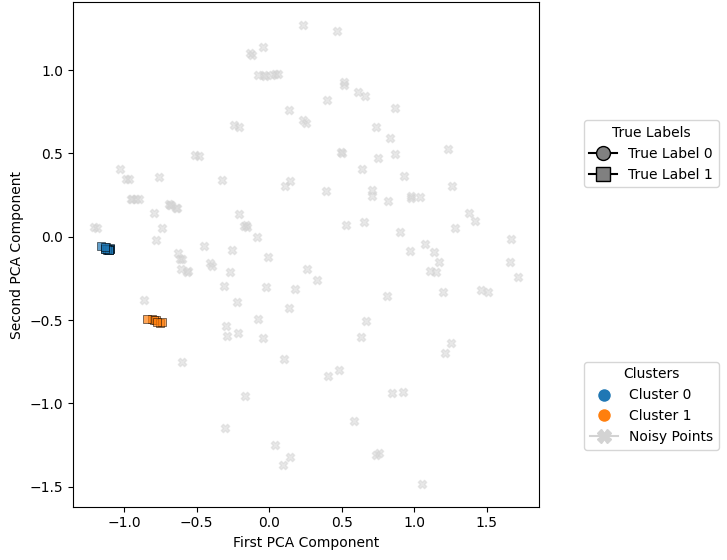
\includegraphics[width=\linewidth]{figures/Optics/hepatitis/br-pca.png}
		\caption{Hepatitis Dataset \\ (\texttt{metric = euclidean}, \\ \texttt{algorithm = brute})}
	\end{subfigure}
	\hfill
	\begin{subfigure}{0.32\textwidth}
		\centering
		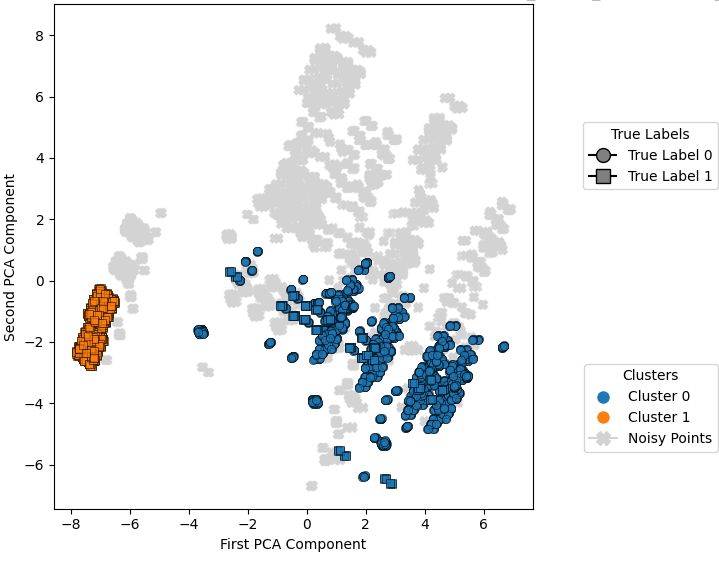
\includegraphics[width=\linewidth]{figures/Optics/mushroom/br-pca.png}
		\caption{Mushroom Dataset \\ (\texttt{metric = euclidean}, \\ \texttt{algorithm = brute})}
	\end{subfigure}
	\hfill
	\begin{subfigure}{0.32\textwidth}
		\centering
		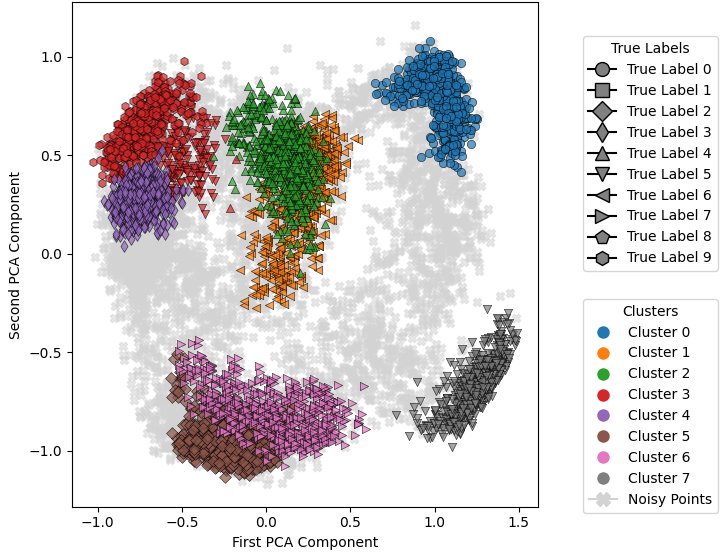
\includegraphics[width=\linewidth]{figures/Optics/pen-based/best_run_CHS_pca.png}
		\caption{Pen-Based Dataset \\ (\texttt{metric = chebyshev}, \\ \texttt{algorithm = brute})}
	\end{subfigure}
	\caption{Visualization of the resulting clusters for each dataset in their two principal components, after applying PCA to each dataset, using some of the best configurations according to the metrics in Table \ref{tab:optics_best_runs}.}
	\label{fig:optics-clusters-br-pca}
\end{figure}


\begin{figure}[H]
	\centering
	\begin{subfigure}{0.32\textwidth}
		\centering
		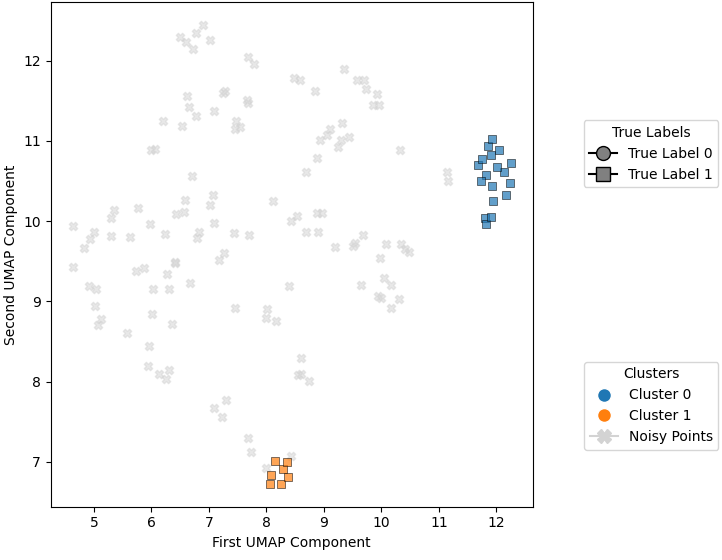
\includegraphics[width=\linewidth]{figures/Optics/hepatitis/br-umap.png}
		\caption{Hepatitis Dataset \\ (\texttt{metric = euclidean}, \\ \texttt{algorithm = brute})}
	\end{subfigure}
	\hfill
	\begin{subfigure}{0.32\textwidth}
		\centering
		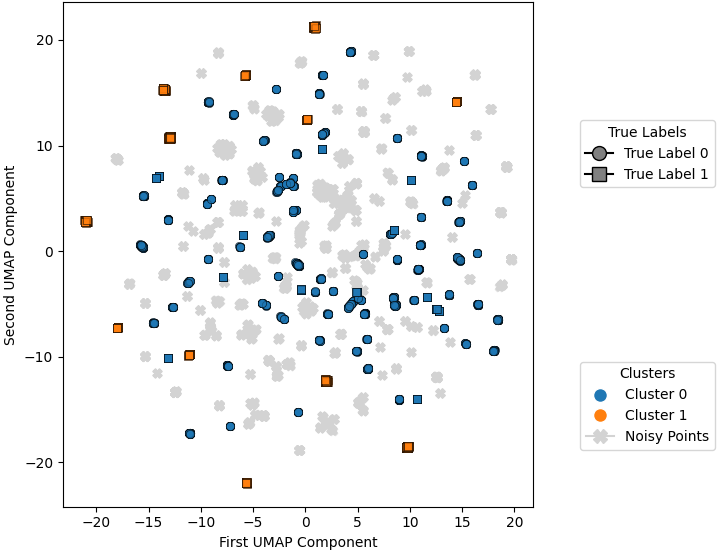
\includegraphics[width=\linewidth]{figures/Optics/mushroom/br-umap.png}
		\caption{Mushroom Dataset \\ (\texttt{metric = euclidean}, \\ \texttt{algorithm = brute})}
	\end{subfigure}
	\hfill
	\begin{subfigure}{0.32\textwidth}
		\centering
		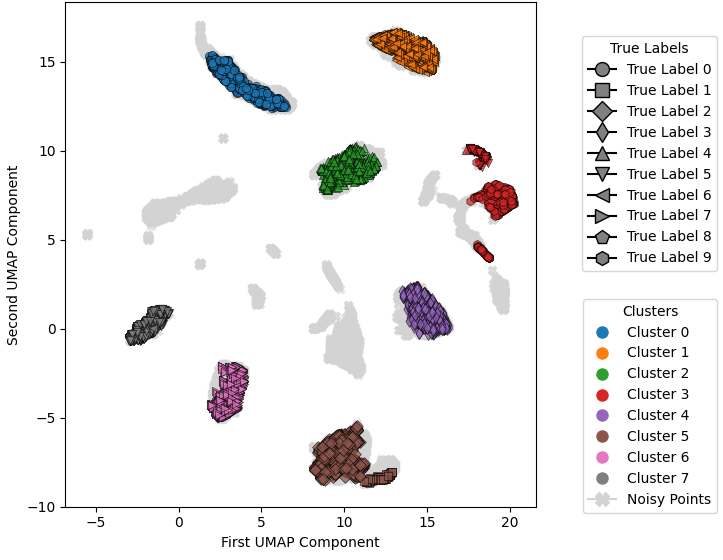
\includegraphics[width=\linewidth]{figures/Optics/pen-based/best_run_CHS_umap.png}
		\caption{Pen-Based Dataset \\ (\texttt{metric = chebyshev}, \\ \texttt{algorithm = brute})}
	\end{subfigure}
	\caption{Visualization of the resulting clusters for each dataset in their two first embedding dimensions, after applying UMAP to each dataset, using some of the best configurations according to the metrics in Table \ref{tab:optics_best_runs}.}
	\label{fig:optics-clusters-br-umap}
\end{figure}